\documentclass[12pt,a4paper]{article}

% ─── Packages ───────────────────────────────────────────────────────────────
\usepackage[margin=2.5cm]{geometry}
\usepackage{amsmath, amssymb, amsthm, mathtools}
\usepackage{braket}          % Dirac notation
\usepackage{physics}         % \abs, \norm, \pdv, etc.
\usepackage{quantikz}        % quantum circuit diagrams
\usepackage{tikz}
\usetikzlibrary{positioning, arrows.meta, shapes, decorations.pathreplacing}
\usepackage{xcolor}
\usepackage{tcolorbox}
\tcbuselibrary{theorems, skins, breakable, listings}
\usepackage{hyperref}
\usepackage{cleveref}
\usepackage{enumitem}
\usepackage{booktabs}
\usepackage{array}
\usepackage{caption}
\usepackage{subcaption}
\usepackage{fancyhdr}
\usepackage{titlesec}
\usepackage{mdframed}
\usepackage{mathrsfs}
% identity via amsfonts
\usepackage{pgfplots}
\pgfplotsset{compat=1.18}
\usepackage{algorithm}
\usepackage{algpseudocode}
\usepackage{multicol}
\usepackage{microtype}

% ─── Colors ─────────────────────────────────────────────────────────────────
\definecolor{qblue}{RGB}{0, 90, 160}
\definecolor{qgreen}{RGB}{0, 130, 80}
\definecolor{qred}{RGB}{180, 30, 30}
\definecolor{qpurple}{RGB}{100, 0, 150}
\definecolor{qorange}{RGB}{200, 100, 0}
\definecolor{lightblue}{RGB}{220, 235, 255}
\definecolor{lightgreen}{RGB}{220, 245, 230}
\definecolor{lightyellow}{RGB}{255, 252, 220}
\definecolor{lightred}{RGB}{255, 230, 230}
\definecolor{lightpurple}{RGB}{240, 225, 255}
\definecolor{darkgray}{RGB}{50, 50, 50}
\definecolor{midgray}{RGB}{120,120,120}

% ─── Hyperref setup ──────────────────────────────────────────────────────────
\hypersetup{
  colorlinks = true,
  linkcolor  = qblue,
  citecolor  = qgreen,
  urlcolor   = qpurple,
  pdftitle   = {Quantum Phase Estimation: A Comprehensive Lecture},
  pdfauthor  = {Quantum Computing Course},
}

% ─── Section formatting ──────────────────────────────────────────────────────
\titleformat{\section}[block]
  {\large\bfseries\color{qblue}}
  {\thesection}{1em}{}[{\color{qblue}\titlerule[0.8pt]}]

\titleformat{\subsection}[block]
  {\normalsize\bfseries\color{qblue!80!black}}
  {\thesubsection}{1em}{}

\titleformat{\subsubsection}[runin]
  {\normalsize\bfseries\color{qpurple}}
  {\thesubsubsection}{1em}{}[.\ ]

% ─── Header / Footer ─────────────────────────────────────────────────────────
\pagestyle{fancy}
\fancyhf{}
\fancyhead[L]{\small\color{midgray}\textit{Quantum Computing — Lecture Notes}}
\fancyhead[R]{\small\color{midgray}\textit{Quantum Phase Estimation}}
\fancyfoot[C]{\small\color{midgray}\thepage}
\renewcommand{\headrulewidth}{0.4pt}

% ─── tcolorbox styles ────────────────────────────────────────────────────────
\tcbset{
  theorem/.style={
    enhanced, breakable,
    colback=lightblue, colframe=qblue,
    fonttitle=\bfseries, separator sign={\ $\blacktriangleright$},
    attach boxed title to top left={yshift=-2mm, xshift=4mm},
    boxed title style={colback=qblue, colframe=qblue!60!black},
    top=4mm,
  },
  definition/.style={
    enhanced, breakable,
    colback=lightgreen, colframe=qgreen,
    fonttitle=\bfseries, separator sign={\ $\blacktriangleright$},
    attach boxed title to top left={yshift=-2mm, xshift=4mm},
    boxed title style={colback=qgreen, colframe=qgreen!60!black},
    top=4mm,
  },
  insight/.style={
    enhanced, breakable,
    colback=lightyellow, colframe=qorange,
    fonttitle=\bfseries\color{qorange},
    title={$\bigstar$\ Insight},
    top=2mm, left=4mm,
  },
  warning/.style={
    enhanced, breakable,
    colback=lightred, colframe=qred,
    fonttitle=\bfseries\color{qred},
    title={$\blacktriangle$\ Common Pitfall},
    top=2mm, left=4mm,
  },
  example/.style={
    enhanced, breakable,
    colback=lightpurple, colframe=qpurple,
    fonttitle=\bfseries,
    separator sign={\ $\blacktriangleright$},
    attach boxed title to top left={yshift=-2mm, xshift=4mm},
    boxed title style={colback=qpurple, colframe=qpurple!60!black},
    top=4mm,
  },
  summary/.style={
    enhanced, breakable,
    colback=darkgray!5, colframe=darkgray,
    fonttitle=\bfseries,
    title={Summary},
    top=2mm,
  },
}

% ─── Theorem environments ────────────────────────────────────────────────────
\newtcbtheorem[number within=section]{theorem}{Theorem}{theorem}{thm}
\newtcbtheorem[number within=section]{lemma}{Lemma}{theorem}{lem}
\newtcbtheorem[number within=section]{corollary}{Corollary}{theorem}{cor}
\newtcbtheorem[number within=section]{definition}{Definition}{definition}{def}
\newtcbtheorem[number within=section]{proposition}{Proposition}{theorem}{prop}

% ─── Maths macros ────────────────────────────────────────────────────────────
\newcommand{\C}{\mathbb{C}}
\newcommand{\R}{\mathbb{R}}
\newcommand{\Z}{\mathbb{Z}}
\newcommand{\N}{\mathbb{N}}
\newcommand{\Id}{\mathbb{1}}
\newcommand{\QPE}{\textsc{QPE}}
\newcommand{\QFT}{\textsc{QFT}}
\newcommand{\IQFT}{\textsc{QFT}^{-1}}
\newcommand{\cU}{c\text{-}U}
\newcommand{\e}{\mathrm{e}}
\newcommand{\ii}{\mathrm{i}}
\newcommand{\bigO}{\mathcal{O}}
\renewcommand{\vec}[1]{\boldsymbol{#1}}
\providecommand{\Tr}{}
\renewcommand{\Tr}{\operatorname{Tr}}
\DeclareMathOperator{\spn}{span}

% Controlled-U gate shorthand
\newcommand{\cUk}{c\text{-}U^{2^k}}

% Phase shorthand
\providecommand{\phase}[1]{e^{2\pi \ii #1}}

% ─── Document ────────────────────────────────────────────────────────────────
\begin{document}

% ============================================================================
%   TITLE PAGE
% ============================================================================
\begin{titlepage}
  \centering
  \vspace*{1.5cm}

  {\color{qblue}\rule{\linewidth}{1.5pt}}
  \vspace{0.4cm}

  {\Huge\bfseries\color{qblue} Quantum Phase Estimation}\\[0.5em]
  {\Large\bfseries\color{qblue!70!black} A Complete and Comprehensive Lecture}

  \vspace{0.3cm}
  {\color{qblue}\rule{\linewidth}{1.5pt}}

  \vspace{1.5cm}

  \begin{tcolorbox}[colback=lightblue, colframe=qblue, width=0.85\linewidth,
      sharp corners, boxrule=1pt]
    \centering
    \textbf{Course:} Quantum Computing\\
    \textbf{Level:} Graduate / Advanced Undergraduate\\[0.3em]
    \textit{Prerequisites: Linear algebra, Dirac notation, basic quantum gates,\\
            quantum Fourier transform at a conceptual level.}
  \end{tcolorbox}

  \vspace{1.5cm}

  \begin{tcolorbox}[colback=lightyellow, colframe=qorange, width=0.85\linewidth,
      sharp corners, boxrule=1pt, title={\bfseries What You Will Learn},
      fonttitle=\bfseries\color{qorange}]
    \begin{enumerate}[leftmargin=*, label=\textbf{\arabic*.}]
      \item The \emph{eigenvalue / phase problem} and why it matters.
      \item How controlled-unitary gates encode phase information.
      \item The structure of the QPE circuit from first principles.
      \item The Quantum Fourier Transform (QFT) as a phase decoder.
      \item Precision, success probability, and error analysis.
      \item A fully worked numerical example — step by step.
      \item Real-world applications: VQE, Shor's algorithm, quantum simulation.
    \end{enumerate}
  \end{tcolorbox}

  \vfill
  {\large\color{midgray} Quantum Computing — Lecture Notes}
\end{titlepage}

% ============================================================================
%   TABLE OF CONTENTS
% ============================================================================
\tableofcontents
\newpage

% ============================================================================
%  SECTION 1 — MOTIVATION AND BIG PICTURE
% ============================================================================
\section{Motivation: Why Eigenvalues Matter in Quantum Computing}
\label{sec:motivation}

\subsection{The Central Problem}

Many of the most important problems in science and engineering reduce to
\emph{eigenvalue problems}.  In chemistry, the ground-state energy of a
molecule is the smallest eigenvalue of its Hamiltonian.  In number theory,
the period of a function (the key to factoring) is related to eigenvalues of
a unitary operator.  In linear systems, stability is governed by eigenvalues.

Classically, finding eigenvalues of an $N \times N$ matrix costs at least
$\bigO(N^2)$ time and often much more.  For quantum systems, $N$ grows
\emph{exponentially} in the number of particles — making the classical
approach completely infeasible.

\begin{tcolorbox}[insight]
  Quantum Phase Estimation (\QPE) solves a specific version of the eigenvalue
  problem:\ given a unitary operator $U$ and (approximately) one of its
  eigenstates $\Ket{\psi}$, estimate the corresponding eigenvalue
  $e^{2\pi \ii \varphi}$ to $n$ bits of precision using only
  $\bigO(n)$ applications of controlled-$U$.  This is exponentially faster
  than any known classical algorithm for the same task.
\end{tcolorbox}

\subsection{The Eigenvalue of a Unitary Operator}

Recall from linear algebra:

\begin{definition}{Unitary Operator \& Its Eigenvalues}{}
  An operator $U$ on $\C^N$ is \textbf{unitary} if $U^\dagger U = U U^\dagger = \Id$.
  A (non-zero) vector $\Ket{\psi}$ is an \textbf{eigenstate} of $U$ with
  \textbf{eigenvalue} $\lambda$ if
  \[
    U\Ket{\psi} = \lambda \Ket{\psi}.
  \]
  Because $U$ is unitary, every eigenvalue satisfies $|\lambda| = 1$, so we
  may write
  \[
    \lambda = e^{2\pi \ii \varphi}, \quad \varphi \in [0,1).
  \]
  The real number $\varphi$ is called the \textbf{phase} of the eigenvalue.
\end{definition}

\medskip

The constraint $|\lambda|=1$ deserves a moment of thought.  If $U\Ket{\psi}=\lambda\Ket{\psi}$, then
\[
  \|\lambda\Ket{\psi}\|^2 = |\lambda|^2\|\Ket{\psi}\|^2
  \;\overset{U \text{ unitary}}{=}\;
  \|U\Ket{\psi}\|^2 = \|\Ket{\psi}\|^2,
\]
which forces $|\lambda|=1$.  Therefore every eigenvalue of every unitary lives on
the complex unit circle, completely characterised by a single real number $\varphi$.

\begin{tcolorbox}[insight]
  \textbf{Rephrasing the goal:}\ QPE finds $\varphi$ given $U$ and $\Ket{\psi}$.
  Every quantum algorithm that claims exponential speedup via QPE ultimately
  reduces its hard problem to: \emph{"find this phase"}.
\end{tcolorbox}

\subsection{Running Example Setup}
\label{subsec:running}

Throughout this lecture we will use the following concrete example, which is
small enough to trace by hand yet rich enough to illustrate every subtlety.

\begin{tcolorbox}[example, title={Running Example: the $T$ gate}]
  Consider the single-qubit \textbf{$T$ gate}:
  \[
    T = \begin{pmatrix} 1 & 0 \\ 0 & e^{i\pi/4} \end{pmatrix}.
  \]
  Its eigenvalues are $1$ (eigenvector $\Ket{0}$) and $e^{i\pi/4}$
  (eigenvector $\Ket{1}$).  Writing the second eigenvalue as
  $e^{2\pi \ii \varphi}$:
  \[
    e^{2\pi \ii \varphi} = e^{i\pi/4}
    \;\Longrightarrow\;
    2\pi\varphi = \frac{\pi}{4}
    \;\Longrightarrow\;
    \varphi = \frac{1}{8}.
  \]
  So we will run QPE with $U=T$ and $\Ket{\psi}=\Ket{1}$, and we hope to
  read out $\varphi = 1/8 = 0.001_2$ (binary).  We will use $n=3$ ancilla
  qubits for the phase register.
\end{tcolorbox}

\newpage

% ============================================================================
%  SECTION 2 — PREREQUISITES AND NOTATION
% ============================================================================
\section{Prerequisites and Notation}
\label{sec:prereqs}

Even though students in this course know the basics, it is worth fixing
notation precisely — small sign or convention errors propagate and spoil the
final result.

\subsection{The Computational Basis and Dirac Notation}

An $n$-qubit \textbf{computational basis state} is written $\Ket{j}$ where
$j \in \{0,1,\ldots,2^n-1\}$ is the decimal value of the binary string.  The
binary string is ordered from \emph{most significant to least significant} bit
from left to right:
\[
  \Ket{j} = \Ket{j_{n-1} j_{n-2} \cdots j_1 j_0},
  \quad j = \sum_{k=0}^{n-1} j_k 2^k.
\]

\subsection{Binary Fractions}

A crucial convenience: define the binary fraction notation
\[
  0.j_1 j_2 \cdots j_n = \sum_{k=1}^{n} \frac{j_k}{2^k}.
\]
So for instance $0.101_2 = 1/2 + 0 + 1/8 = 5/8$.  The phase $\varphi$ will
often be expressed exactly as such a fraction.

\subsection{The Quantum Fourier Transform (QFT)}
\label{subsec:qft}

QPE \emph{uses} the QFT as a sub-routine, so we must understand it well.

\begin{definition}{Quantum Fourier Transform}{}
  The $n$-qubit \textbf{Quantum Fourier Transform} is the unitary operator
  whose action on computational basis states is
  \[
    \QFT\Ket{j} = \frac{1}{\sqrt{2^n}}
    \sum_{k=0}^{2^n-1} e^{2\pi \ii jk/2^n}\Ket{k}.
  \]
  In product form (essential for circuit implementation):
  \[
    \QFT\Ket{j_1 j_2 \cdots j_n}
    = \frac{1}{\sqrt{2^n}}
      \Bigl(\Ket{0}+e^{2\pi \ii 0.j_n}\Ket{1}\Bigr)
      \otimes
      \Bigl(\Ket{0}+e^{2\pi \ii 0.j_{n-1}j_n}\Ket{1}\Bigr)
      \otimes \cdots \otimes
      \Bigl(\Ket{0}+e^{2\pi \ii 0.j_1 j_2 \cdots j_n}\Ket{1}\Bigr).
  \]
\end{definition}

\medskip

\begin{tcolorbox}[insight]
  \textbf{Why the product form matters:}\ it shows that each qubit of the QFT
  output carries one bit of the binary fraction $0.j_1 j_2 \cdots j_n$.  This
  is the key to understanding how QPE decodes the phase: the phase
  $\varphi$ gets encoded into exactly this product form, and the inverse QFT
  then reads it out.
\end{tcolorbox}

\subsection{Controlled-Unitary Gates}

\begin{definition}{Controlled-$U$ Gate}{}
  Given a unitary $U$ acting on $m$ qubits, the \textbf{controlled-$U$} gate
  $\cU$ acts on $m+1$ qubits (one control, $m$ target) as:
  \[
    \cU \;\Ket{c}\Ket{x} =
    \begin{cases}
      \Ket{0}\Ket{x} & \text{if } c=0, \\
      \Ket{1} U\Ket{x} & \text{if } c=1.
    \end{cases}
  \]
  More compactly, $\cU = \Ket{0}\!\Bra{0}\otimes \Id + \Ket{1}\!\Bra{1}\otimes U$.
\end{definition}

\medskip
Now observe what happens when the control qubit is in superposition and the
target is an eigenstate $U\Ket{\psi}=e^{2\pi \ii \varphi}\Ket{\psi}$:
\begin{align}
  \cU \;\frac{\Ket{0}+\Ket{1}}{\sqrt{2}}\Ket{\psi}
  &= \frac{\Ket{0}\Id\Ket{\psi}+\Ket{1}U\Ket{\psi}}{\sqrt{2}} \notag \\
  &= \frac{\Ket{0}\Ket{\psi}+e^{2\pi \ii \varphi}\Ket{1}\Ket{\psi}}{\sqrt{2}} \notag \\
  &= \frac{\Ket{0}+e^{2\pi \ii \varphi}\Ket{1}}{\sqrt{2}}\otimes\Ket{\psi}.
  \label{eq:phase_kickback}
\end{align}

\begin{tcolorbox}[insight]
  \textbf{Phase Kickback.}\ Equation~\eqref{eq:phase_kickback} shows that the
  phase $e^{2\pi \ii \varphi}$ has been \emph{kicked back} onto the control qubit,
  leaving $\Ket{\psi}$ unchanged.  This is the single most important mechanism
  in QPE, and it is why QPE uses controlled-$U^{2^k}$ gates rather than any
  other gate.
\end{tcolorbox}

\newpage

% ============================================================================
%  SECTION 3 — THE QPE CIRCUIT: STRUCTURE AND INTUITION
% ============================================================================
\section{The QPE Circuit: Structure and Deep Intuition}
\label{sec:circuit}

\subsection{Circuit Overview}

QPE uses two registers:
\begin{itemize}[leftmargin=*]
  \item \textbf{Phase register} (ancilla): $n$ qubits, initialised to $\Ket{0}^{\otimes n}$.
        These will store the $n$-bit estimate of $\varphi$.
  \item \textbf{Eigenstate register}: $m$ qubits holding $\Ket{\psi}$,
        the eigenstate of $U$.
\end{itemize}

The circuit has three stages:
\begin{enumerate}[label=\textbf{Stage \arabic*.}]
  \item \textbf{Superposition:} Apply $H^{\otimes n}$ to the phase register.
  \item \textbf{Controlled rotations:} Apply $c\text{-}U^{2^k}$ for
        $k = 0, 1, \ldots, n-1$.
  \item \textbf{Inverse QFT:} Apply $\IQFT$ to the phase register, then measure.
\end{enumerate}

\subsection{The Circuit Diagram}

\[
\begin{quantikz}[row sep=0.35cm, column sep=0.5cm]
  \lstick{$\ket{0}$} & \gate{H} & \ctrl{4} & \qw      & \qw      & \cdots & \qw      & \qw & \gate[4]{\QFT^{-1}} & \meter{} \\
  \lstick{$\ket{0}$} & \gate{H} & \qw      & \ctrl{3} & \qw      & \cdots & \qw      & \qw &                     & \meter{} \\
  \lstick{\vdots}    &          &          &          & \ddots   &        &          &     &                     & \\
  \lstick{$\ket{0}$} & \gate{H} & \qw      & \qw      & \qw      & \cdots & \ctrl{1} & \qw &                     & \meter{} \\
  \lstick{$\ket{\psi}$} & \qwbundle{m} & \gate{U^{2^{n-1}}} & \gate{U^{2^{n-2}}} & \gate{U^{2^{n-3}}} & \cdots & \gate{U^{2^{0}}} & \qw & \qw & \qw \\
\end{quantikz}
\]

\medskip
\noindent\textbf{Reading the diagram:} The top-most ancilla qubit controls
$U^{2^{n-1}}$ (the highest power), while the bottom ancilla qubit controls
$U^{2^0}=U$.  After all controlled gates, the $n$ ancilla qubits undergo the
inverse QFT, and then each is measured in the computational basis.

\subsection{Stage 1 — Creating Superposition (Why Hadamard?)}
\label{subsec:stage1}

After applying $H^{\otimes n}$ to $\Ket{0}^{\otimes n}$, the phase register becomes
\[
  H^{\otimes n}\Ket{0}^{\otimes n}
  = \bigotimes_{k=0}^{n-1} \frac{\Ket{0}+\Ket{1}}{\sqrt{2}}
  = \frac{1}{\sqrt{2^n}} \sum_{j=0}^{2^n-1} \Ket{j}.
\]

\begin{tcolorbox}[insight]
  \textbf{Why superposition first?}  We want the controlled gates to be able
  to \emph{simultaneously probe} $U$ raised to all powers $2^0, 2^1, \ldots,
  2^{n-1}$.  Without superposition, each qubit can only be in state $\Ket{0}$
  and the controlled gates would do nothing.  The Hadamard creates a superposition
  so that when phase kickback occurs, it applies to the $\Ket{1}$ branch of
  each qubit, encoding phase information into the relative phases of the
  superposition.
\end{tcolorbox}

\subsection{Stage 2 — Controlled-$U^{2^k}$ Gates (Why These Powers?)}
\label{subsec:stage2}

Let qubit $k$ (counting from 0 at the \emph{bottom}) of the phase register
control the gate $U^{2^k}$.  Before this stage, the full system state is:
\[
  \frac{1}{\sqrt{2^n}}\sum_{j=0}^{2^n-1}\Ket{j}\otimes\Ket{\psi}.
\]
After all $n$ controlled gates, using the phase kickback from
Eq.~\eqref{eq:phase_kickback} applied $n$ times (once for each qubit), the
state becomes:
\begin{align}
  &\frac{1}{\sqrt{2^n}}\sum_{j=0}^{2^n-1} e^{2\pi \ii \varphi j}\Ket{j}\otimes\Ket{\psi}.
  \label{eq:after_controlled}
\end{align}

\textbf{Derivation of Eq.~\eqref{eq:after_controlled}.}\ Consider qubit $k$
(which controls $U^{2^k}$).  In the state $\sum_j \Ket{j}$, qubit $k$
contributes a factor of $\Ket{0}+\Ket{1}$ (ignoring normalisation).  After
the controlled-$U^{2^k}$ with eigenstate $\Ket{\psi}$:
\[
  \Ket{0}+\Ket{1} \;\longmapsto\; \Ket{0}+e^{2\pi \ii \varphi \cdot 2^k}\Ket{1}.
\]
This happens independently for each qubit $k = 0, 1, \ldots, n-1$, so the
combined state of the phase register is the tensor product:
\begin{align*}
  &\bigotimes_{k=0}^{n-1}\frac{\Ket{0}+e^{2\pi \ii \varphi 2^k}\Ket{1}}{\sqrt{2}}
  = \frac{1}{\sqrt{2^n}} \sum_{j=0}^{2^n-1}
      \prod_{k=0}^{n-1} e^{2\pi \ii \varphi 2^k j_k} \Ket{j} \\
  &= \frac{1}{\sqrt{2^n}} \sum_{j=0}^{2^n-1}
      e^{2\pi \ii \varphi \sum_{k=0}^{n-1} 2^k j_k} \Ket{j}
  = \frac{1}{\sqrt{2^n}} \sum_{j=0}^{2^n-1}
      e^{2\pi \ii \varphi j}\Ket{j}.
\end{align*}

The last step uses $j = \sum_{k=0}^{n-1} 2^k j_k$.

\begin{tcolorbox}[insight]
  \textbf{Why powers of 2?}  The binary expansion of $j$ is exactly
  $j = \sum_k 2^k j_k$.  By choosing the $k$-th gate to apply $U^{2^k}$, we
  ensure that the accumulated phase for basis state $\Ket{j}$ is exactly
  $e^{2\pi \ii \varphi j}$ — precisely the form required by the Quantum
  Fourier Transform!  Any other choice of exponents would not reproduce this
  clean structure.
\end{tcolorbox}

\subsection{Stage 3 — Inverse QFT (Why It Decodes the Phase)}
\label{subsec:stage3}

After Stage 2, the phase register is in the state (ignoring $\Ket{\psi}$):
\[
  \Ket{\Phi} = \frac{1}{\sqrt{2^n}}\sum_{j=0}^{2^n-1} e^{2\pi \ii \varphi j}\Ket{j}.
\]

This is almost exactly the QFT of a computational basis state!  Recall:
\[
  \QFT\Ket{f} = \frac{1}{\sqrt{2^n}}\sum_{j=0}^{2^n-1} e^{2\pi \ii fj/2^n}\Ket{j}.
\]

Comparing: if $\varphi = f/2^n$ (i.e., $\varphi$ is an exact $n$-bit binary
fraction), then $\Ket{\Phi} = \QFT\Ket{f}$, which means
\[
  \IQFT\Ket{\Phi} = \Ket{f},
\]
and measuring gives $f$ with certainty, from which $\varphi = f/2^n$.

\begin{tcolorbox}[insight]
  \textbf{The inverse QFT as a decoder.}\ Stage 2 prepared a state that is
  the QFT of a "spike" at frequency $f = \varphi \cdot 2^n$.  Applying the
  inverse QFT converts the frequency-domain state back to the time domain,
  yielding (approximately) the computational basis state $\Ket{f}$.  This is
  the quantum analogue of the inverse FFT extracting a dominant frequency from
  a signal.
\end{tcolorbox}

\begin{tcolorbox}[warning]
  This exact analysis only works when $\varphi$ is an exact $n$-bit binary
  fraction (i.e., $\varphi = f/2^n$ for integer $f$).  In general,
  $\varphi$ need not be exactly representable, and we get a probability
  distribution peaked near $\lfloor \varphi \cdot 2^n \rceil$.  Section~\ref{sec:precision}
  analyses this in detail.
\end{tcolorbox}

\newpage

% ============================================================================
%  SECTION 4 — STEP-BY-STEP DERIVATION
% ============================================================================
\section{Complete Step-by-Step Circuit Analysis}
\label{sec:derivation}

We now trace the circuit \emph{algebraically}, step by step, for a general
$n$-qubit phase register.

\subsection{Initial State}

\[
  \Ket{\Psi_0} = \underbrace{\Ket{0}^{\otimes n}}_{\text{phase register}} \otimes
  \underbrace{\Ket{\psi}}_{\text{eigenstate}}.
\]

\subsection{After Hadamard Layer}

Apply $H$ to each of the $n$ phase qubits independently:
\[
  \Ket{\Psi_1}
  = H^{\otimes n}\Ket{0}^{\otimes n}\otimes\Ket{\psi}
  = \frac{1}{\sqrt{2^n}}\sum_{j=0}^{2^n-1}\Ket{j}\otimes\Ket{\psi}.
\]

\subsection{After Controlled-$U^{2^k}$ Gates}

\begin{proposition}{}{}
  After applying controlled-$U^{2^k}$ (control: qubit $k$, target: eigenstate
  register) for $k = n-1, n-2, \ldots, 0$, the state is:
  \[
    \Ket{\Psi_2}
    = \frac{1}{\sqrt{2^n}}\sum_{j=0}^{2^n-1} e^{2\pi \ii \varphi j}\Ket{j}\otimes\Ket{\psi}.
  \]
\end{proposition}

\begin{proof}
  We prove this by showing the action on each qubit separately.  Write the
  phase register in the tensor product basis.  Qubit $k$ (from LSB) is in
  state $\tfrac{1}{\sqrt{2}}(\Ket{0}+\Ket{1})$.  The controlled-$U^{2^k}$
  acts as:
  \[
    \frac{\Ket{0}+\Ket{1}}{\sqrt{2}}\otimes\Ket{\psi}
    \;\longmapsto\;
    \frac{\Ket{0}\cdot\Id\Ket{\psi}+\Ket{1}\cdot U^{2^k}\Ket{\psi}}{\sqrt{2}}
    = \frac{\Ket{0}+e^{2\pi \ii \varphi 2^k}\Ket{1}}{\sqrt{2}}\otimes\Ket{\psi}.
  \]
  Since different qubits control different (non-overlapping) gates acting on
  the same eigenstate register (and $\Ket{\psi}$ is unchanged), the $n$-qubit
  state after all controlled gates factors as:
  \[
    \Ket{\Psi_2}
    = \bigotimes_{k=0}^{n-1}
        \frac{\Ket{0}+e^{2\pi \ii \varphi 2^k}\Ket{1}}{\sqrt{2}}
      \otimes\Ket{\psi}.
  \]
  Expanding the tensor product, the coefficient of $\Ket{j} = \Ket{j_{n-1}\cdots j_0}$
  is
  \[
    \frac{1}{\sqrt{2^n}}
    \prod_{k=0}^{n-1} \Bigl(e^{2\pi \ii \varphi 2^k}\Bigr)^{j_k}
    = \frac{1}{\sqrt{2^n}} e^{2\pi \ii \varphi \sum_k 2^k j_k}
    = \frac{1}{\sqrt{2^n}} e^{2\pi \ii \varphi j}. \qedhere
  \]
\end{proof}

\subsection{After Inverse QFT}

We apply $\IQFT$ to the phase register.  The inverse QFT acts as:
\[
  \IQFT\Ket{j} = \frac{1}{\sqrt{2^n}}\sum_{k=0}^{2^n-1} e^{-2\pi \ii jk/2^n}\Ket{k}.
\]
By linearity:
\begin{align}
  \Ket{\Psi_3}
  &= \IQFT\left[\frac{1}{\sqrt{2^n}}\sum_{j=0}^{2^n-1} e^{2\pi \ii \varphi j}\Ket{j}\right]
     \otimes\Ket{\psi} \notag \\
  &= \frac{1}{\sqrt{2^n}}\sum_{j=0}^{2^n-1} e^{2\pi \ii \varphi j}\left[
       \frac{1}{\sqrt{2^n}}\sum_{k=0}^{2^n-1} e^{-2\pi \ii jk/2^n}\Ket{k}
     \right]\otimes\Ket{\psi} \notag \\
  &= \frac{1}{2^n}\sum_{k=0}^{2^n-1}\left[
       \sum_{j=0}^{2^n-1} e^{2\pi \ii j(\varphi - k/2^n)}
     \right]\Ket{k}\otimes\Ket{\psi}.
  \label{eq:after_iqft}
\end{align}

\begin{definition}{Probability Amplitude}{}
  From Eq.~\eqref{eq:after_iqft}, the probability amplitude of measuring
  outcome $k$ is:
  \[
    \alpha_k = \frac{1}{2^n}\sum_{j=0}^{2^n-1} e^{2\pi \ii j(\varphi - k/2^n)},
  \]
  and the corresponding probability is $P(k) = |\alpha_k|^2$.
\end{definition}

\medskip

\subsubsection{Case 1: $\varphi$ is an exact $n$-bit binary fraction}

If $\varphi = f/2^n$ for some integer $f\in\{0,\ldots,2^n-1\}$, then:
\[
  \alpha_k = \frac{1}{2^n}\sum_{j=0}^{2^n-1} e^{2\pi \ii j(f-k)/2^n}.
\]
This is a geometric series.  For $k\neq f$:
\[
  \alpha_k = \frac{1}{2^n}\cdot\frac{1-e^{2\pi \ii (f-k)}}{1-e^{2\pi \ii (f-k)/2^n}}=0,
\]
because $(f-k)$ is a nonzero integer so $e^{2\pi \ii (f-k)}=1$ and
$e^{2\pi \ii (f-k)/2^n}\neq 1$.  For $k=f$, all terms equal 1, so
$\alpha_f = 1$.  Therefore:
\[
  \boxed{P(k) = \begin{cases} 1 & k = f, \\ 0 & k \neq f. \end{cases}}
\]
Measurement gives $f$ with certainty, and we recover $\varphi = f/2^n$ exactly!

\subsubsection{Case 2: $\varphi$ is not exactly representable}

Let $b = \lfloor \varphi \cdot 2^n \rceil$ be the nearest integer (ties broken
by rounding down).  Write $\delta = \varphi - b/2^n \in (-1/2^{n+1}, 1/2^{n+1}]$.
Then:
\[
  P(b) = \left|\frac{1}{2^n}\sum_{j=0}^{2^n-1}e^{2\pi \ii j\delta}\right|^2
  = \frac{1}{4^n}\left|\frac{\sin(\pi 2^n \delta)}{\sin(\pi\delta)}\right|^2.
\]

For $\delta=0$ (exact case) this equals 1.  For $|\delta|\leq 1/2^{n+1}$
(worst case), one can show $P(b)\geq 4/\pi^2 \approx 0.405$.

\begin{tcolorbox}[insight]
  Even in the worst case (phase exactly halfway between two representable
  values), QPE still succeeds with probability at least $40.5\%$.  Repeating
  the measurement $r$ times and taking the majority vote increases success
  probability to $1-\epsilon$ for any $\epsilon>0$ at a cost of only
  $\bigO(\log(1/\epsilon))$ repetitions.
\end{tcolorbox}

\newpage

% ============================================================================
%  SECTION 5 — PRECISION AND ERROR ANALYSIS
% ============================================================================
\section{Precision, Success Probability, and Error Analysis}
\label{sec:precision}

\subsection{Precision of $n$ Ancilla Qubits}

With $n$ ancilla qubits, the phase register can represent $2^n$ distinct
values: $\{0, 1/2^n, 2/2^n, \ldots, (2^n-1)/2^n\}$.  Thus the \emph{resolution}
of QPE is $1/2^n$.

\begin{theorem}{QPE Precision Guarantee}{}
  Let $\varphi\in[0,1)$ be the true phase.  With $n$ ancilla qubits, QPE
  produces an estimate $\tilde{\varphi}=k/2^n$ satisfying
  \[
    |\tilde{\varphi}-\varphi| \leq \frac{1}{2^n}
  \]
  with probability at least $1 - \epsilon$ by using
  \[
    n = \left\lceil\log_2\!\left(\frac{1}{\epsilon} + \frac{1}{2}\right)\right\rceil
    + \left\lceil\log_2\!\left(\frac{1}{\epsilon'}\right)\right\rceil
  \]
  qubits, where $\epsilon'$ is the desired error in $\varphi$ and $\epsilon$
  the allowed failure probability.
\end{theorem}

\medskip

A simpler rule of thumb: to get $t$ bits of precision in $\varphi$ with
success probability at least $1-2^{-(s+1)}$, use $n = t + s + 1$ ancilla qubits.

\subsection{The Probability Distribution}

\begin{figure}[h]
\centering
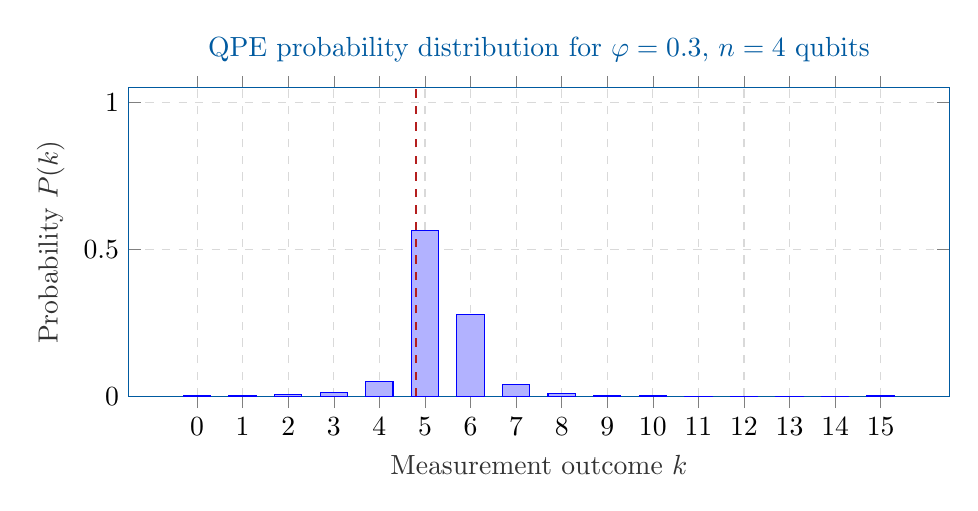
\begin{tikzpicture}
\begin{axis}[
  width=12cm, height=5.5cm,
  xlabel={Measurement outcome $k$},
  ylabel={Probability $P(k)$},
  title={QPE probability distribution for $\varphi=0.3$, $n=4$ qubits},
  xtick={0,1,...,15},
  xticklabels={0,1,2,3,4,5,6,7,8,9,10,11,12,13,14,15},
  ymin=0, ymax=1.05,
  bar width=0.6,
  ybar,
  fill=qblue!50, draw=qblue,
  grid=major, grid style={dashed, gray!30},
  title style={color=qblue},
  xlabel style={color=darkgray},
  ylabel style={color=darkgray},
]
% Precomputed: phi=0.3, n=4 (2^4=16), P(k)=|sum_{j=0}^{15} e^{2pi i j(0.3-k/16)}|^2 / 256
% Dominant outcomes: k=4 (phi*16=4.8 -> round to 5), k=5
% Computed numerically:
\addplot coordinates {
  (0, 0.0034) (1, 0.0041) (2, 0.0064) (3, 0.0136) (4, 0.0522)
  (5, 0.5657) (6, 0.2795) (7, 0.0419) (8, 0.0105) (9, 0.0040)
  (10, 0.0019) (11, 0.0012) (12, 0.0009) (13, 0.0008) (14, 0.0010)
  (15, 0.0017)
};
\draw[qred, thick, dashed] (axis cs:4.8, 0) -- (axis cs:4.8, 1.05)
  node[above, font=\small, color=qred] {$\varphi\cdot 2^n=4.8$};
\end{axis}
\end{tikzpicture}
\caption{Probability distribution over measurement outcomes for $\varphi=0.3$ and
  $n=4$ qubits.  The peak at $k=5$ (with $P\approx56.6\%$) gives estimate
  $\tilde\varphi=5/16=0.3125$, which is the nearest representable value to
  $0.3$.  The second peak at $k=4$ has $P\approx5.2\%$, giving
  $\tilde\varphi=0.25$.}
\label{fig:dist}
\end{figure}

\subsection{Circuit Complexity}

\begin{table}[h]
\centering
\caption{QPE gate complexity with $n$ ancilla qubits and controlled-$U$
  implementable in $g$ gates.}
\begin{tabular}{@{}lcc@{}}
\toprule
\textbf{Component} & \textbf{Gate count} & \textbf{Notes} \\
\midrule
Hadamard layer     & $n$ & One per ancilla qubit \\
Controlled-$U^{2^k}$ gates & $\sum_{k=0}^{n-1} g\cdot 2^k = g(2^n-1)$ & If implemented by repetition \\
Controlled-$U^{2^k}$ gates & $\bigO(n\cdot g)$ & If $U^{2^k}$ computed by squaring \\
Inverse QFT        & $\bigO(n^2)$ & Exact; $\bigO(n\log n)$ approximate \\
Measurement        & $n$ & \\
\midrule
\textbf{Total}     & $\bigO(n^2 + ng)$ & \\
\bottomrule
\end{tabular}
\label{tab:complexity}
\end{table}

\begin{tcolorbox}[insight]
  The key to QPE's power is \textbf{repeated squaring}: computing $U^{2^k}$
  from $U$ takes only $k$ multiplications, so $U^{2^{n-1}}$ requires only
  $n-1$ squarings.  This is why QPE costs $\bigO(n)$ applications of $U$
  (by squaring) rather than $\bigO(2^n)$ (by repetition), achieving an
  exponential speedup in the number of oracle calls.
\end{tcolorbox}

\newpage

% ============================================================================
%  SECTION 6 — FULLY WORKED NUMERICAL EXAMPLE
% ============================================================================
\section{Fully Worked Numerical Example: The $T$ Gate}
\label{sec:example}

We now execute the complete QPE circuit for our running example from
Section~\ref{subsec:running}.

\begin{tcolorbox}[example, title={Setup}]
  \begin{itemize}[leftmargin=*]
    \item $U = T = \begin{pmatrix}1&0\\0&e^{i\pi/4}\end{pmatrix}$
    \item Eigenstate: $\Ket{\psi} = \Ket{1}$, eigenvalue $e^{i\pi/4}=e^{2\pi i/8}$
    \item True phase: $\varphi = 1/8 = 0.001_2$
    \item Ancilla qubits: $n = 3$ (so $2^3 = 8$ representable values)
    \item Phase register: qubits $q_2, q_1, q_0$ (MSB to LSB)
    \item Expected measurement outcome: $f = \lfloor 1/8 \cdot 8 \rceil = 1$,
          i.e., $\Ket{001}$
  \end{itemize}
\end{tcolorbox}

\subsection{Step 0: Powers of $T$}

We need $T^{2^0}=T$, $T^{2^1}=T^2$, and $T^{2^2}=T^4$.  Let's compute these:
\[
  T = \begin{pmatrix}1&0\\0&e^{i\pi/4}\end{pmatrix},\qquad
  T^2 = \begin{pmatrix}1&0\\0&e^{i\pi/2}\end{pmatrix}
       = \begin{pmatrix}1&0\\0&i\end{pmatrix}\quad(= S \text{ gate}),
\]
\[
  T^4 = \begin{pmatrix}1&0\\0&e^{i\pi}\end{pmatrix}
       = \begin{pmatrix}1&0\\0&-1\end{pmatrix}\quad(= Z \text{ gate}).
\]

\medskip
Checking on the eigenstate $\Ket{1}$:
\[
  T^{2^k}\Ket{1} = e^{i\pi 2^k/4}\Ket{1}
  = e^{2\pi i \cdot 2^k /8}\Ket{1},
\]
confirming phase kickback will give factor $e^{2\pi i \cdot 2^k/8}$ on the $k$-th control qubit.

\subsection{Step 1: Initial State}

\[
  \Ket{\Psi_0} = \Ket{0}\Ket{0}\Ket{0}\otimes\Ket{1}
  \equiv \Ket{000}\Ket{1}.
\]

Written out with qubit labels (MSB $q_2$, LSB $q_0$):
\[
  q_2 = \Ket{0},\quad q_1 = \Ket{0},\quad q_0 = \Ket{0},\quad
  \text{eigenstate} = \Ket{1}.
\]

\subsection{Step 2: Apply Hadamard to Each Ancilla}

\[
  H\Ket{0} = \frac{\Ket{0}+\Ket{1}}{\sqrt{2}}.
\]
After $H^{\otimes 3}$:
\[
  \Ket{\Psi_1}
  = \frac{\Ket{0}+\Ket{1}}{\sqrt{2}}
    \otimes
    \frac{\Ket{0}+\Ket{1}}{\sqrt{2}}
    \otimes
    \frac{\Ket{0}+\Ket{1}}{\sqrt{2}}
    \otimes\Ket{1}.
\]

Expanding the phase register (8 terms):
\[
  \Ket{\Psi_1}
  = \frac{1}{\sqrt{8}}\bigl(
    \Ket{000}+\Ket{001}+\Ket{010}+\Ket{011}
    +\Ket{100}+\Ket{101}+\Ket{110}+\Ket{111}
  \bigr)\otimes\Ket{1}.
\]

\subsection{Step 3: Apply Controlled-$U^4$ (qubit $q_2$ controls $T^4 = Z$)}

$q_2$ is the most significant qubit.  When $q_2=1$, apply $Z$ to $\Ket{1}$:
\[
  Z\Ket{1} = -\Ket{1} = e^{i\pi}\Ket{1} = e^{2\pi i \cdot 4/8}\Ket{1}.
\]

The phase $e^{2\pi i/8\cdot 4}$ kicks back onto the $\Ket{1}$ component of $q_2$:
\[
  q_2: \frac{\Ket{0}+\Ket{1}}{\sqrt{2}}
  \;\longmapsto\;
  \frac{\Ket{0}+e^{2\pi i\cdot 4/8}\Ket{1}}{\sqrt{2}}
  = \frac{\Ket{0}+e^{i\pi}\Ket{1}}{\sqrt{2}}
  = \frac{\Ket{0}-\Ket{1}}{\sqrt{2}}.
\]

After this gate ($q_1, q_0$ unchanged):
\[
  \Ket{\Psi_{2a}}
  = \frac{\Ket{0}-\Ket{1}}{\sqrt{2}}
    \otimes
    \frac{\Ket{0}+\Ket{1}}{\sqrt{2}}
    \otimes
    \frac{\Ket{0}+\Ket{1}}{\sqrt{2}}
    \otimes\Ket{1}.
\]

\subsection{Step 4: Apply Controlled-$U^2$ (qubit $q_1$ controls $T^2 = S$)}

$S\Ket{1} = i\Ket{1} = e^{i\pi/2}\Ket{1} = e^{2\pi i \cdot 2/8}\Ket{1}$.

Phase kick on $q_1$:
\[
  q_1: \frac{\Ket{0}+\Ket{1}}{\sqrt{2}}
  \;\longmapsto\;
  \frac{\Ket{0}+e^{2\pi i\cdot 2/8}\Ket{1}}{\sqrt{2}}
  = \frac{\Ket{0}+i\Ket{1}}{\sqrt{2}}.
\]

After this gate:
\[
  \Ket{\Psi_{2b}}
  = \frac{\Ket{0}-\Ket{1}}{\sqrt{2}}
    \otimes
    \frac{\Ket{0}+i\Ket{1}}{\sqrt{2}}
    \otimes
    \frac{\Ket{0}+\Ket{1}}{\sqrt{2}}
    \otimes\Ket{1}.
\]

\subsection{Step 5: Apply Controlled-$U^1$ (qubit $q_0$ controls $T$)}

$T\Ket{1} = e^{i\pi/4}\Ket{1} = e^{2\pi i \cdot 1/8}\Ket{1}$.

Phase kick on $q_0$:
\[
  q_0: \frac{\Ket{0}+\Ket{1}}{\sqrt{2}}
  \;\longmapsto\;
  \frac{\Ket{0}+e^{2\pi i \cdot 1/8}\Ket{1}}{\sqrt{2}}
  = \frac{\Ket{0}+e^{i\pi/4}\Ket{1}}{\sqrt{2}}.
\]

After all controlled gates, the state is:
\begin{align}
  \Ket{\Psi_2}
  &= \underbrace{\frac{\Ket{0}-\Ket{1}}{\sqrt{2}}}_{q_2}
     \otimes
     \underbrace{\frac{\Ket{0}+i\Ket{1}}{\sqrt{2}}}_{q_1}
     \otimes
     \underbrace{\frac{\Ket{0}+e^{i\pi/4}\Ket{1}}{\sqrt{2}}}_{q_0}
     \otimes\Ket{1} \notag \\
  &= \frac{1}{\sqrt{8}}\sum_{j=0}^{7} e^{2\pi i j/8}\Ket{j}\otimes\Ket{1},
  \label{eq:psi2_example}
\end{align}
where the last equality uses our general formula with $\varphi = 1/8$.  Let us
verify this by expanding.  The coefficient of $\Ket{j} = \Ket{j_2 j_1 j_0}$ is:
\[
  (-1)^{j_2} \cdot i^{j_1} \cdot e^{i\pi j_0/4}
  = e^{i\pi j_2} \cdot e^{i\pi j_1/2} \cdot e^{i\pi j_0/4}
  = e^{i\pi(4j_2+2j_1+j_0)/4}
  = e^{2\pi i j /8},
\]
confirming Eq.~\eqref{eq:psi2_example}.

\subsection{Step 6: Apply Inverse QFT}

We must apply the 3-qubit $\IQFT$ to the phase register.  Since
$\varphi = 1/8 = 1/2^3$ is exactly representable with 3 bits ($f=1$), the
inverse QFT should give us $\Ket{001}$ with probability 1.

Let us verify using the formula for $\IQFT$:
\begin{align*}
  \IQFT\Ket{\Psi_2}
  &= \IQFT\left[\frac{1}{\sqrt{8}}\sum_{j=0}^{7}e^{2\pi i j/8}\Ket{j}\right]
     \otimes\Ket{1} \\
  &= \frac{1}{8}\sum_{k=0}^{7}\left[\sum_{j=0}^{7}e^{2\pi ij(1/8-k/8)}\right]\Ket{k}
     \otimes\Ket{1} \\
  &= \frac{1}{8}\sum_{k=0}^{7}\left[\sum_{j=0}^{7}e^{2\pi ij(1-k)/8}\right]\Ket{k}
     \otimes\Ket{1}.
\end{align*}

For each $k$, the inner sum is a geometric series with ratio $\omega^{1-k}$ where
$\omega = e^{2\pi i/8}$:
\[
  S_k = \sum_{j=0}^{7}\omega^{j(1-k)} =
  \begin{cases}
    8 & \text{if } 1-k \equiv 0 \pmod{8}, \text{ i.e., } k=1, \\
    0 & \text{otherwise}.
  \end{cases}
\]

Therefore:
\[
  \boxed{
  \Ket{\Psi_3} = \Ket{001}\otimes\Ket{1}.
  }
\]

\subsection{Step 7: Measurement}

Measuring the phase register yields $\Ket{001}$ with probability 1.
Interpreting the 3-bit string as a binary fraction:
\[
  \tilde{\varphi} = 0.001_2 = \frac{0}{2}+\frac{0}{4}+\frac{1}{8} = \frac{1}{8}.
\]

\begin{tcolorbox}[example, title={Result}]
  \[
    \boxed{\tilde\varphi = \frac{1}{8} = \varphi \checkmark}
  \]
  QPE recovers the phase exactly because $\varphi=1/8$ is representable as
  a 3-bit binary fraction.  The eigenstate register is left in $\Ket{1}$,
  undisturbed.
\end{tcolorbox}

\subsection{Summarising the Numerical Steps}

\begin{table}[h]
\centering
\caption{State of the phase register at each stage of QPE for the $T$ gate example.}
\begin{tabular}{@{}clll@{}}
\toprule
\textbf{Stage} & \textbf{$q_2$} & \textbf{$q_1$} & \textbf{$q_0$} \\
\midrule
0. Init & $\Ket{0}$ & $\Ket{0}$ & $\Ket{0}$ \\
1. After $H$ & $\frac{\Ket{0}+\Ket{1}}{\sqrt2}$ & $\frac{\Ket{0}+\Ket{1}}{\sqrt2}$ & $\frac{\Ket{0}+\Ket{1}}{\sqrt2}$ \\
2a. After $c$-$T^4$ & $\frac{\Ket{0}-\Ket{1}}{\sqrt2}$ & $\frac{\Ket{0}+\Ket{1}}{\sqrt2}$ & $\frac{\Ket{0}+\Ket{1}}{\sqrt2}$ \\
2b. After $c$-$T^2$ & $\frac{\Ket{0}-\Ket{1}}{\sqrt2}$ & $\frac{\Ket{0}+i\Ket{1}}{\sqrt2}$ & $\frac{\Ket{0}+\Ket{1}}{\sqrt2}$ \\
2c. After $c$-$T$ & $\frac{\Ket{0}-\Ket{1}}{\sqrt2}$ & $\frac{\Ket{0}+i\Ket{1}}{\sqrt2}$ & $\frac{\Ket{0}+e^{i\pi/4}\Ket{1}}{\sqrt2}$ \\
3. After $\IQFT$ & $\Ket{0}$ & $\Ket{0}$ & $\Ket{1}$ \\
4. Measurement & $0$ & $0$ & $1$ \\
\bottomrule
\end{tabular}
\end{table}

\newpage

% ============================================================================
%  SECTION 7 — WHAT IF PHI IS NOT EXACTLY REPRESENTABLE?
% ============================================================================
\section{Non-Exact Phase: A Second Example}
\label{sec:nonexact}

To solidify understanding, let us briefly analyse what happens when $\varphi$
is \emph{not} representable exactly.  Take $U$ with $\varphi = 1/3$ and $n=3$
ancilla qubits.

\subsection{After the Controlled Gates}

The general formula gives:
\[
  \Ket{\Psi_2} = \frac{1}{\sqrt{8}}\sum_{j=0}^{7}e^{2\pi ij/3}\Ket{j}\otimes\Ket{\psi}.
\]

\subsection{Probabilities After Inverse QFT}

The probability of measuring outcome $k$ is:
\[
  P(k) = \frac{1}{64}\left|\sum_{j=0}^7 e^{2\pi ij(1/3-k/8)}\right|^2.
\]

Computing numerically ($\varphi\cdot 8 = 8/3 \approx 2.667$, so nearest
integers are $k=3$ and $k=2$):

\begin{center}
\begin{tabular}{@{}cccc@{}}
\toprule
$k$ & $\tilde{\varphi}=k/8$ & Error $|\tilde\varphi-1/3|$ & $P(k)$ \\
\midrule
2 & 0.250 & 0.0833 & $\approx 0.188$ \\
3 & 0.375 & 0.0417 & $\approx 0.600$ \\
4 & 0.500 & 0.1667 & $\approx 0.051$ \\
\bottomrule
\end{tabular}
\end{center}

\begin{tcolorbox}[insight]
  With probability $\approx 60\%$, we measure $k=3$ giving $\tilde\varphi =
  3/8 = 0.375$, which approximates $1/3\approx 0.333$ with error $\approx 0.042 < 1/8$.
  The guarantee holds: the error is at most $1/2^n = 1/8$.  Adding more
  ancilla qubits shrinks the resolution and improves the approximation.
\end{tcolorbox}

\newpage

% ============================================================================
%  SECTION 8 — THE INVERSE QFT CIRCUIT IN DETAIL
% ============================================================================
\section{The Inverse QFT Circuit}
\label{sec:iqft}

The QFT/IQFT is itself a quantum algorithm, not a single gate.  Since QPE
uses the IQFT, students must understand its structure.

\subsection{The QFT Circuit}

The $n$-qubit QFT is implemented using:
\begin{itemize}[leftmargin=*]
  \item $n$ Hadamard gates.
  \item $\frac{n(n-1)}{2}$ controlled-phase gates $R_k = \begin{pmatrix}1&0\\0&e^{2\pi i/2^k}\end{pmatrix}$.
  \item $\lfloor n/2\rfloor$ SWAP gates (to reverse bit order).
\end{itemize}

\[
\begin{quantikz}[row sep=0.4cm, column sep=0.6cm]
\lstick{$\ket{j_1}$} & \gate{H} & \gate{R_2} & \gate{R_3} & \qw & \cdots & & \gate{R_n} & \qw & \swap{3} & \qw \\
\lstick{$\ket{j_2}$} & \qw & \ctrl{-1} & \qw & \gate{H} & \cdots & & \gate{R_{n-1}} & \qw & \qw & \qw \\
\lstick{\vdots} & & & & & \ddots & & & & & \\
\lstick{$\ket{j_n}$} & \qw & \qw & \qw & \qw & \cdots & & \ctrl{-3} & \gate{H} & \targX{} & \qw
\end{quantikz}
\]

The IQFT is simply the \emph{reverse circuit with all phase angles negated}:
replace each $R_k$ by $R_k^\dagger = \begin{pmatrix}1&0\\0&e^{-2\pi i/2^k}\end{pmatrix}$
and run the circuit in reverse.

\subsection{Why Does the QFT Work?}

The QFT maps $\Ket{j_1 j_2 \cdots j_n}$ to
\[
  \frac{1}{\sqrt{2^n}}
  \Bigl(\Ket{0}+e^{2\pi i 0.j_n}\Ket{1}\Bigr)
  \otimes
  \Bigl(\Ket{0}+e^{2\pi i 0.j_{n-1}j_n}\Ket{1}\Bigr)
  \otimes\cdots\otimes
  \Bigl(\Ket{0}+e^{2\pi i 0.j_1 j_2\cdots j_n}\Ket{1}\Bigr).
\]

The $k$-th factor depends only on the last $k$ bits of $j$.  This is achieved by:
\begin{enumerate}[leftmargin=*]
  \item \textbf{Hadamard on qubit 1}: produces $\Ket{0}+e^{2\pi i 0.j_1}\Ket{1}$.
  \item \textbf{Controlled-$R_2$ from qubit 2}: adds $e^{2\pi i j_2/4}$ when qubit 2 is 1,
        giving $\Ket{0}+e^{2\pi i 0.j_1 j_2}\Ket{1}$.
  \item \textbf{Continue}: each controlled-$R_k$ from qubit $k$ appends one more bit
        to the binary fraction in the exponent.
  \item \textbf{Repeat for each qubit}, then \textbf{swap} to reverse bit order.
\end{enumerate}

\subsection{QFT Example: 3-qubit QFT of $\Ket{001}$}
\label{subsec:qft_example}

We verify that $\QFT\Ket{001}$ gives the state prepared by QPE (confirming
that $\IQFT$ will recover $\Ket{001}$).

$\Ket{001}$: $j_1=0, j_2=0, j_3=1$, so $j = 1$.

\[
  \QFT\Ket{001}
  = \frac{1}{\sqrt{8}}\sum_{k=0}^{7}e^{2\pi i \cdot 1\cdot k/8}\Ket{k}
  = \frac{1}{\sqrt{8}}\sum_{k=0}^{7}e^{2\pi i k/8}\Ket{k}.
\]

This matches $\Ket{\Psi_2}$ from our QPE example exactly, confirming that
$\IQFT\Ket{\Psi_2} = \Ket{001}$.

\newpage

% ============================================================================
%  SECTION 9 — GENERAL INITIAL STATE (MIXED EIGENSTATES)
% ============================================================================
\section{QPE With a General (Mixed Eigenstate) Input}
\label{sec:general}

So far we assumed $\Ket{\psi}$ is a \emph{pure eigenstate}.  What if we
input a superposition of eigenstates?

\subsection{Superposition of Eigenstates}

Let $U\Ket{u_j}=e^{2\pi i\varphi_j}\Ket{u_j}$ for $j=0,1,\ldots$, and
suppose the eigenstate register is initialised to
$\Ket{\chi}=\sum_j c_j \Ket{u_j}$ (with $\sum_j|c_j|^2=1$).

By linearity, the QPE circuit evolves:
\[
  \Ket{0}^{\otimes n}\otimes\Ket{\chi}
  = \sum_j c_j \Ket{0}^{\otimes n}\otimes\Ket{u_j}
  \;\;\xrightarrow{\text{QPE}}\;\;
  \sum_j c_j \Ket{\tilde\varphi_j}\otimes\Ket{u_j},
\]
where $\Ket{\tilde\varphi_j}$ is the phase-register state peaked at $\varphi_j$.

\subsection{Measurement Outcomes}

After measurement of the phase register, with probability $|c_j|^2$ we measure
$\tilde\varphi_j$ (approximately) and the eigenstate register collapses to
$\Ket{u_j}$.  Thus:
\begin{itemize}[leftmargin=*]
  \item Each run of QPE samples one eigenphase, with probability $|c_j|^2$.
  \item After measurement, the eigenstate register is left in the corresponding
        eigenstate.
  \item If one eigenstate dominates ($|c_0|^2 \approx 1$), QPE reliably
        returns $\varphi_0$.
\end{itemize}

\begin{tcolorbox}[insight]
  This is precisely how QPE is used in the \textbf{Variational Quantum
  Eigensolver (VQE)}: one prepares a trial state $\Ket{\chi}$ that has
  large overlap with the ground state $\Ket{u_0}$ of the Hamiltonian, then
  QPE reliably estimates $\varphi_0$ (the ground-state energy).  The better
  the trial state, the more reliable the energy estimate.
\end{tcolorbox}

\newpage

% ============================================================================
%  SECTION 10 — APPLICATIONS
% ============================================================================
\section{Applications of Quantum Phase Estimation}
\label{sec:applications}

QPE is arguably the most important quantum subroutine.  Here we survey its
most significant applications.

\subsection{Shor's Algorithm for Integer Factorisation}

Shor's algorithm~\cite{shor1994} factors an integer $N$ in polynomial time.
The key step: find the \emph{period} $r$ of the function $f(x)=a^x \bmod N$.
This is done by constructing the unitary
\[
  U_a\Ket{x} = \Ket{ax \bmod N}
\]
and noting that the eigenvalues of $U_a$ are $e^{2\pi i s/r}$ for
$s=0,1,\ldots,r-1$.  QPE extracts these eigenvalues, from which $r$ is
recovered by the continued-fraction algorithm.  Factoring then follows from
$r$.  The overall complexity is $\bigO((\log N)^3)$, compared to the best
known classical algorithm's $\bigO(\exp((\log N)^{1/3}(\log\log N)^{2/3}))$.

\subsection{Quantum Simulation}

Given a Hamiltonian $H$, the time-evolution operator $U = e^{-iHt}$ is unitary.
Its eigenvalues are $e^{-iE_k t}$ where $E_k$ are energy eigenvalues.  QPE on
$U$ therefore extracts the energy spectrum of $H$, enabling:
\begin{itemize}[leftmargin=*]
  \item Calculation of molecular ground-state energies (quantum chemistry).
  \item Simulation of condensed-matter systems (band structures, phase transitions).
  \item Lattice gauge theory simulations.
\end{itemize}

\subsection{HHL Algorithm for Linear Systems}

The Harrow-Hassidim-Lloyd (HHL) algorithm~\cite{harrow2009} solves $A\vec{x}=\vec{b}$
in $\bigO(\log N)$ time (under certain conditions) using QPE to extract the
eigenvalues $\lambda_j$ of $A$, then applies their reciprocals $1/\lambda_j$
to invert $A$.

\subsection{Quantum Counting}

QPE can count the number of solutions to a search problem.  The Grover
iterator $G$ has eigenvalues $e^{\pm 2i\theta}$ where $\sin^2\theta = M/N$
($M$ = solutions, $N$ = search space size).  QPE on $G$ extracts $\theta$,
from which $M$ is computed.

\begin{table}[h]
\centering
\caption{Summary of QPE applications.}
\begin{tabular}{@{}lll@{}}
\toprule
\textbf{Application} & \textbf{Unitary $U$} & \textbf{Phase encodes} \\
\midrule
Shor's factoring & $U_a\Ket{x}=\Ket{ax\bmod N}$ & Period $r$ \\
Quantum chemistry & $e^{-iHt}$ & Energy eigenvalue $E_k$ \\
HHL linear systems & $e^{iAt}$ & Eigenvalue $\lambda_j$ of $A$ \\
Quantum counting & Grover iterator $G$ & Number of solutions $M$ \\
\bottomrule
\end{tabular}
\end{table}

\newpage

% ============================================================================
%  SECTION 11 — PRACTICAL CONSIDERATIONS
% ============================================================================
\section{Practical Considerations for QPE}
\label{sec:practical}

\subsection{Implementing Controlled-$U^{2^k}$ in Practice}

The main cost of QPE comes from the controlled-$U^{2^k}$ gates.  For large
$k$, $2^k$ can be astronomically large.  Two strategies:

\begin{enumerate}[label=\textbf{\arabic*.}, leftmargin=*]
  \item \textbf{Repeated squaring.}\ Compute $U^{2^k}$ by squaring $k$ times:
        $U^{2^k} = (U^{2^{k-1}})^2$.  Total cost: $\bigO(n)$ matrix
        multiplications, each costing $\bigO(m^3)$ classically or $\bigO(m)$
        queries quantumly.
  \item \textbf{Problem-specific structure.}\ For quantum simulation,
        $e^{-iHt\cdot 2^k} = e^{-iH(t2^k)}$.  This can be implemented using
        Trotter decompositions applied to $2^k t$ instead of $t$.
\end{enumerate}

\subsection{Ancilla Qubit Count vs Precision}

The trade-off is stark:
\begin{itemize}[leftmargin=*]
  \item Each additional ancilla qubit \emph{doubles} the precision.
  \item For chemistry applications, chemical accuracy requires $|\tilde\varphi - \varphi| \lesssim 10^{-3}$, demanding $n \geq 10$ ancilla qubits.
  \item Each ancilla qubit adds one layer of $n$ controlled gates, increasing circuit depth.
\end{itemize}

\subsection{Noise and Error Mitigation}

On current NISQ devices, every gate has a non-trivial error rate $\epsilon_g$.
A QPE circuit with $\bigO(n^2 + ng)$ gates has total error $\sim n^2\epsilon_g$,
which grows quickly with precision.  Strategies:
\begin{itemize}[leftmargin=*]
  \item \textbf{Iterative QPE:} Estimate one bit of $\varphi$ at a time using
        a single ancilla qubit, iterating $n$ times.  Reduces circuit depth at
        the cost of more measurements.
  \item \textbf{Hadamard test:} Estimate real and imaginary parts of
        $\Bra{\psi}U^k\Ket{\psi}$ separately, then use classical post-processing.
  \item \textbf{Error-mitigation techniques:} Zero-noise extrapolation,
        probabilistic error cancellation.
\end{itemize}

\subsection{Iterative QPE}
\label{subsec:iqpe}

Iterative QPE (IQPE) estimates $\varphi$ one bit at a time, using only a
\emph{single} ancilla qubit.  The idea: the LSB of $\varphi$ is the phase of
$U^{2^{n-1}}\Ket{\psi}$.  After measuring the LSB, a classical feedback
corrects the phase before extracting the next bit.  This reduces the qubit
count from $n+m$ to $1+m$ at the cost of $n$ sequential rounds of measurement.

\begin{algorithm}[h]
\caption{Iterative QPE}
\begin{algorithmic}[1]
\Require Oracle for $U$, eigenstate $\Ket{\psi}$, number of bits $n$
\Ensure Approximation $\tilde\varphi = 0.\omega_1\omega_2\cdots\omega_n$ to $\varphi$
\State $\Phi \gets 0$ \Comment{Classical feedback angle}
\For{$k = n, n-1, \ldots, 1$}
  \State Prepare ancilla $\Ket{+} = H\Ket{0}$
  \State Apply controlled-$U^{2^{k-1}}$ to $\Ket{\psi}$ with ancilla as control
  \State Apply $R_Z(-\Phi)$ to ancilla \Comment{Undo accumulated phase}
  \State Apply $H$ to ancilla
  \State Measure ancilla, store result as $\omega_{n-k+1} \in \{0,1\}$
  \State $\Phi \gets (\Phi + \omega_{n-k+1}\pi)/2$
\EndFor
\State \Return $\tilde\varphi = \sum_{k=1}^n \omega_k / 2^k$
\end{algorithmic}
\end{algorithm}

\newpage

% ============================================================================
%  SECTION 12 — COMPLETE ALGORITHM SUMMARY
% ============================================================================
\section{Complete Algorithm Summary}
\label{sec:summary}

\begin{tcolorbox}[summary]
  \textbf{Quantum Phase Estimation — Complete Description}

  \medskip
  \textbf{Input:} Black-box unitary $U$; (approximate) eigenstate $\Ket{\psi}$;
  desired precision $n$ bits.

  \medskip
  \textbf{Output:} $\tilde\varphi \in \{0, 1/2^n, \ldots, (2^n-1)/2^n\}$
  such that $|\tilde\varphi - \varphi| \leq 1/2^n$ with probability $\geq 1-\delta$.

  \medskip
  \textbf{Algorithm:}
  \begin{enumerate}[leftmargin=*]
    \item Initialise: $\Ket{0}^{\otimes n}\otimes\Ket{\psi}$.
    \item Apply $H^{\otimes n}$ to phase register.
    \item For $k=0,\ldots,n-1$: apply controlled-$U^{2^k}$ (control: qubit $k$).
    \item Apply $\IQFT$ to phase register.
    \item Measure phase register; output $\tilde\varphi = (\text{result})/2^n$.
  \end{enumerate}

  \medskip
  \textbf{Cost:}
  \begin{itemize}[leftmargin=*]
    \item $n + \bigO(n^2)$ gates (Hadamards + IQFT).
    \item $\bigO(n)$ queries to controlled-$U$ (with squaring).
    \item Error $\leq 1/2^n$ with probability $\geq 4/\pi^2 \approx 40.5\%$ (single shot).
    \item Error $\leq 1/2^n$ with probability $\geq 1-\delta$ using
          $\bigO(\log(1/\delta))$ repetitions.
  \end{itemize}
\end{tcolorbox}

\bigskip

\begin{figure}[h]
\centering
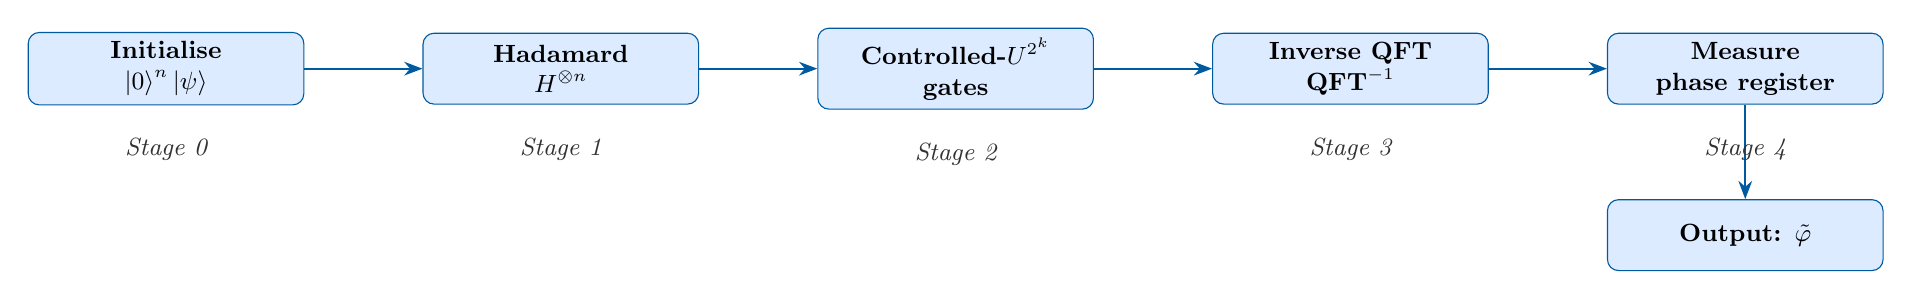
\begin{tikzpicture}[
  node distance=1.5cm,
  box/.style={draw=qblue, fill=lightblue, rounded corners, minimum width=3.5cm,
              minimum height=0.9cm, align=center, font=\small\bfseries},
  arrow/.style={-Stealth, qblue, thick},
  label/.style={font=\small\itshape, color=darkgray},
]
\node[box] (init) {Initialise\\$\Ket{0}^n\Ket{\psi}$};
\node[box, right=of init] (had) {Hadamard\\$H^{\otimes n}$};
\node[box, right=of had] (cu) {Controlled-$U^{2^k}$\\gates};
\node[box, right=of cu] (iqft) {Inverse QFT\\$\IQFT$};
\node[box, right=of iqft] (meas) {Measure\\phase register};
\node[box, below=1.2cm of meas] (out) {Output: $\tilde\varphi$};

\draw[arrow] (init) -- (had);
\draw[arrow] (had) -- (cu);
\draw[arrow] (cu) -- (iqft);
\draw[arrow] (iqft) -- (meas);
\draw[arrow] (meas) -- (out);

\node[label, below=0.3cm of init] {Stage 0};
\node[label, below=0.3cm of had] {Stage 1};
\node[label, below=0.3cm of cu] {Stage 2};
\node[label, below=0.3cm of iqft] {Stage 3};
\node[label, below=0.3cm of meas] {Stage 4};
\end{tikzpicture}
\caption{High-level flow of the QPE algorithm.}
\end{figure}

\newpage

% ============================================================================
%  SECTION 13 — COMMON MISTAKES AND HOW TO AVOID THEM
% ============================================================================
\section{Common Mistakes and How to Avoid Them}
\label{sec:mistakes}

\begin{tcolorbox}[warning]
  \textbf{Mistake 1: Confusing $\varphi$ with the eigenvalue.}\ The
  eigenvalue is $e^{2\pi i\varphi}$; QPE estimates $\varphi \in [0,1)$,
  not $e^{2\pi i\varphi}$.  Always remember to compute $e^{2\pi i \cdot (\text{measured value})}$ if you need the eigenvalue.
\end{tcolorbox}

\begin{tcolorbox}[warning]
  \textbf{Mistake 2: Wrong bit ordering.}\ There are two common conventions
  for which qubit is MSB vs LSB.  The convention in this lecture (qubit 0 =
  LSB = controls $U^{2^0}$) is standard in Nielsen \& Chuang.  Some texts
  use the opposite convention.  A circuit built with the wrong convention will
  output the \emph{bit-reversal} of the correct answer, which is incorrect but
  a valid binary fraction — so the error is silent!
\end{tcolorbox}

\begin{tcolorbox}[warning]
  \textbf{Mistake 3: Forgetting the QFT bit-reversal swap.}\ The standard
  QFT circuit produces output with bits in reverse order.  The SWAP gates at
  the end correct this.  If you implement the QFT without SWAPs and use it as
  the forward transform, you must also implement the inverse without SWAPs;
  they must be consistent.
\end{tcolorbox}

\begin{tcolorbox}[warning]
  \textbf{Mistake 4: Assuming $\Ket{\psi}$ is always an exact eigenstate.}\
  In practice, the input state often has imperfect overlap with the target
  eigenstate.  Section~\ref{sec:general} shows that QPE still works but
  probabilistically samples among the eigenstates with probabilities given by
  the squared overlaps.
\end{tcolorbox}

\begin{tcolorbox}[warning]
  \textbf{Mistake 5: Conflating circuit depth with oracle query count.}\
  QPE requires $n$ controlled-$U$ oracle calls (by squaring).  But each
  controlled-$U^{2^k}$ may itself require $\bigO(2^k)$ elementary gates if
  $U$ has no special structure.  The oracle complexity and gate complexity
  can differ exponentially.
\end{tcolorbox}

\newpage

% ============================================================================
%  SECTION 14 — REVIEW QUESTIONS AND EXERCISES
% ============================================================================
\section{Review Questions and Exercises}
\label{sec:exercises}

\subsection{Conceptual Questions}

\begin{enumerate}[label=\textbf{Q\arabic*.}, leftmargin=*]
  \item \textbf{Phase kickback.}\ Explain in your own words why the phase
        $e^{2\pi i\varphi}$ is kicked back onto the control qubit and not
        the target qubit.  What property of $\Ket{\psi}$ is essential?

  \item \textbf{Why Hadamard first?}\ If we omit the initial Hadamard layer
        and apply the controlled gates to $\Ket{0}^{\otimes n}$, what state
        do we get?  Why does the inverse QFT then fail to give us $\varphi$?

  \item \textbf{Why powers of 2?}\ Suppose we replace the controlled-$U^{2^k}$
        gates with controlled-$U^k$ (powers $1, 2, 3, \ldots, n$).  Does the
        inverse QFT still decode the phase?  Explain.

  \item \textbf{Precision vs qubits.}\ How many ancilla qubits are needed to
        estimate a phase to 6 decimal digits with success probability at least
        $99\%$?

  \item \textbf{The inverse QFT.}\ Why do we apply the \emph{inverse} QFT
        rather than the QFT itself?  What would happen if we applied the
        forward QFT instead?
\end{enumerate}

\subsection{Computational Exercises}

\begin{enumerate}[label=\textbf{E\arabic*.}, leftmargin=*]
  \item \textbf{$Z$ gate.}\ Run QPE on $U=Z$ with eigenstate $\Ket{1}$
        using $n=2$ ancilla qubits.  Trace all states, verify the measurement
        outcome, and extract $\varphi$.

  \item \textbf{$S$ gate.}\ Run QPE on $U=S=\begin{pmatrix}1&0\\0&i\end{pmatrix}$
        with $\Ket{\psi}=\Ket{1}$ and $n=3$ qubits.  The eigenvalue is $i = e^{i\pi/2}$,
        so $\varphi=1/4$.  Verify you recover $\Ket{010}$ (i.e., $2/8=1/4$).

  \item \textbf{Non-exact phase.}\ Set $\varphi = 1/3$ and $n=3$.  Compute
        $P(k)$ for all $k\in\{0,\ldots,7\}$ and verify that $P(3)\geq 4/\pi^2$.

  \item \textbf{Doubled precision.}\ Repeat Exercise E1 with $n=4$ qubits.
        What is the new resolution?  Does the extra qubit change the measurement outcome?

  \item \textbf{Hadamard test.}\ Show that the circuit consisting of
        (a) $H$ on the ancilla, (b) controlled-$U$, (c) $H$ on the ancilla,
        and (d) measurement, gives $P(\text{ancilla}=0) = \tfrac{1}{2}(1+\operatorname{Re}\Bra{\psi}U\Ket{\psi})$.
        How does this relate to QPE?
\end{enumerate}

\subsection{Challenging Problems}

\begin{enumerate}[label=\textbf{C\arabic*.}, leftmargin=*]
  \item \textbf{Success probability lower bound.}\ Prove rigorously that
        $P(b) \geq 4/\pi^2 \approx 0.405$ where $b$ is the nearest integer
        to $\varphi\cdot 2^n$. \emph{Hint:}\ Bound the geometric sum and use
        the inequality $\sin x \leq x$.

  \item \textbf{Boosting success probability.}\ Given a QPE circuit with
        success probability $p \geq 4/\pi^2$, show that repeating $r$ times
        and taking the majority vote gives success probability $\geq 1-e^{-\Omega(r)}$.

  \item \textbf{Shor's period finding.}\ Look up the unitary $U_a$ used in
        Shor's algorithm.  Show that its eigenvalues are $e^{2\pi i s/r}$ for
        $s=0,\ldots,r-1$, where $r$ is the order of $a \bmod N$.  How does QPE
        extract $r$ from these eigenvalues?

  \item \textbf{Iterative QPE.}\ Implement the IQPE algorithm of
        Section~\ref{subsec:iqpe} in a quantum circuit simulator of your choice.
        Verify it recovers $\varphi = 1/8$ using a single ancilla qubit and $n=3$ rounds.
\end{enumerate}

\newpage

% ============================================================================
%  SECTION 15 — FURTHER READING
% ============================================================================
\section{Further Reading}
\label{sec:reading}

\begin{itemize}[leftmargin=*]
  \item \textbf{Foundational text:}\ Nielsen and Chuang, \textit{Quantum
        Computation and Quantum Information} (Cambridge University Press, 2010),
        Chapter 5.  This is the standard reference; Chapter 5.2 covers QPE
        and 5.3 covers applications.

  \item \textbf{Shor's algorithm:}\ P.W.\ Shor, ``Polynomial-time algorithms
        for prime factorization and discrete logarithms on a quantum computer,''
        SIAM J.\ Comput.\ 26(5), 1997.  Essential reading for seeing QPE in
        action.

  \item \textbf{HHL algorithm:}\ A.W.\ Harrow, A.\ Hassidim, S.\ Lloyd,
        ``Quantum algorithm for linear systems of equations,'' PRL 103(15), 2009.

  \item \textbf{Quantum chemistry:}\ A.\ Aspuru-Guzik et al., ``Simulated quantum
        computation of molecular energies,'' Science 309(5741), 2005.  The first
        paper to propose QPE for quantum chemistry.

  \item \textbf{Iterative QPE:}\ D.\ Kitaev, ``Quantum measurements and the
        abelian stabilizer problem,'' arXiv:quant-ph/9511026, 1995.  The
        original IQPE proposal.

  \item \textbf{Modern review:}\ S.\ McArdle et al., ``Quantum computational
        chemistry,'' Rev.\ Mod.\ Phys.\ 92(1), 2020.  Comprehensive coverage
        of QPE in near-term quantum computing.

  \item \textbf{Qiskit tutorials:}\ \url{https://qiskit.org/learn/} — worked
        QPE implementations in Python with IBM Quantum hardware.

  \item \textbf{Quirk:}\ \url{https://algassert.com/quirk} — a browser-based
        quantum circuit simulator excellent for visualising QPE interactively.
\end{itemize}

\newpage

% ============================================================================
%  SECTION 16 — KEY EQUATIONS CHEAT SHEET
% ============================================================================
\section{Key Equations Cheat Sheet}
\label{sec:cheatsheet}

\begin{tcolorbox}[colback=lightyellow, colframe=qorange, title={\bfseries QPE Quick Reference},
    fonttitle=\bfseries\color{qorange}]

\textbf{Setting:} $U$ unitary, $U\Ket{\psi}=e^{2\pi i\varphi}\Ket{\psi}$, $\varphi\in[0,1)$.

\medskip
\textbf{Phase kickback:}
\[
  c\text{-}U^{2^k}\;\frac{\Ket{0}+\Ket{1}}{\sqrt{2}}\Ket{\psi}
  = \frac{\Ket{0}+e^{2\pi i\varphi 2^k}\Ket{1}}{\sqrt{2}}\Ket{\psi}.
\]

\textbf{State after Stage 2:}
\[
  \frac{1}{\sqrt{2^n}}\sum_{j=0}^{2^n-1}e^{2\pi i\varphi j}\Ket{j}\Ket{\psi}.
\]

\textbf{Probability of outcome $k$:}
\[
  P(k) = \frac{1}{4^n}\left|\sum_{j=0}^{2^n-1}e^{2\pi ij(\varphi-k/2^n)}\right|^2.
\]

\textbf{Exact case} ($\varphi=f/2^n$): $P(f)=1$, all others $0$.

\textbf{Worst-case success:} $P(b)\geq 4/\pi^2\approx 40.5\%$.

\textbf{Resolution:} $|\tilde\varphi-\varphi|\leq 1/2^n$.

\textbf{Gate count:} $\bigO(n^2+ng)$ total, $\bigO(n)$ queries to $U$.

\textbf{QFT:}
$\QFT\Ket{j}=\frac{1}{\sqrt{2^n}}\sum_{k}e^{2\pi ijk/2^n}\Ket{k}$.

\textbf{IQFT:}
$\IQFT\Ket{j}=\frac{1}{\sqrt{2^n}}\sum_{k}e^{-2\pi ijk/2^n}\Ket{k}$.

\end{tcolorbox}

\newpage

% ============================================================================
%  APPENDIX A — GEOMETRIC SERIES COMPUTATION
% ============================================================================
\appendix
\section{Geometric Series Closed Form}
\label{app:geosum}

For the probability amplitude computation, we repeatedly use:

\[
  \sum_{j=0}^{N-1} r^j = \frac{1-r^N}{1-r}, \quad r\neq 1.
\]

With $r = e^{2\pi i\alpha}$ for non-integer $\alpha$:
\[
  \left|\sum_{j=0}^{N-1}e^{2\pi ij\alpha}\right|^2
  = \frac{|1-e^{2\pi iN\alpha}|^2}{|1-e^{2\pi i\alpha}|^2}
  = \frac{\sin^2(\pi N\alpha)}{\sin^2(\pi\alpha)}.
\]

This uses $|1-e^{i\theta}|=2|\sin(\theta/2)|$.

\section{Binary Fraction Expansion}
\label{app:binary}

Any $\varphi\in[0,1)$ has the binary expansion
$\varphi = \sum_{k=1}^{\infty} b_k 2^{-k}$ with $b_k\in\{0,1\}$.
The $n$-bit truncation $f/2^n = \sum_{k=1}^n b_k 2^{-k}$ satisfies
$|\varphi - f/2^n| \leq 2^{-n}$.

\textbf{Conversion examples:}
\begin{center}
\begin{tabular}{@{}cccc@{}}
\toprule
$\varphi$ & Binary & $n$-bit approx $(n=3)$ & Error \\
\midrule
$1/2$   & $0.1$      & $0.100_2=4/8$ & $0$ \\
$1/4$   & $0.01$     & $0.010_2=2/8$ & $0$ \\
$1/8$   & $0.001$    & $0.001_2=1/8$ & $0$ \\
$1/3$   & $0.010101\ldots$ & $0.011_2=3/8$ & $1/24\approx0.042$ \\
$1/5$   & $0.001100\ldots$ & $0.001_2=1/8$ & $3/40=0.075$ \\
\bottomrule
\end{tabular}
\end{center}

\section{Verification of the $T$-Gate Example Using Matrix Multiplication}
\label{app:matrix}

For completeness, we verify the phase-register state after all controlled
gates in the $n=3$, $U=T$ example by direct matrix computation.

The 3-qubit phase register state (ignoring $\Ket{1}$ of the eigenstate
register) just before the IQFT was derived as:
\[
  \Ket{\Psi_2}\text{(phase register)}
  = \frac{1}{\sqrt{8}}\bigl(
    \Ket{000}+e^{i\pi/4}\Ket{001}+i\Ket{010}+ie^{i\pi/4}\Ket{011}
    -\Ket{100}-e^{i\pi/4}\Ket{101}-i\Ket{110}-ie^{i\pi/4}\Ket{111}
  \bigr).
\]

The coefficient vector is $\vec{v} = \frac{1}{\sqrt{8}}[1, \omega, i, i\omega, -1, -\omega, -i, -i\omega]^T$
where $\omega = e^{i\pi/4}$.  Note $\omega = e^{2\pi i/8}$, so the $j$-th
coefficient is $\frac{1}{\sqrt{8}}e^{2\pi i j/8}$, confirming our formula.

Applying the $8\times 8$ inverse DFT matrix $F^{-1}$ (with entries $(F^{-1})_{kj}=\frac{1}{\sqrt{8}}e^{-2\pi ikj/8}$):
\[
  (F^{-1}\vec{v})_k
  = \frac{1}{8}\sum_{j=0}^7 e^{-2\pi ikj/8}\cdot e^{2\pi ij/8}
  = \frac{1}{8}\sum_{j=0}^7 e^{2\pi ij(1-k)/8}
  = \delta_{k,1}.
\]

Therefore $F^{-1}\vec{v} = \vec{e}_1 = [0,1,0,0,0,0,0,0]^T$, corresponding
to the state $\Ket{001}$, confirming our result. $\square$

% ============================================================================
%  REFERENCES (manual, since this is a lecture note)
% ============================================================================
\begin{thebibliography}{9}

\bibitem{nielsen2010}
M.A.\ Nielsen and I.L.\ Chuang,
\textit{Quantum Computation and Quantum Information},
10th anniversary ed., Cambridge University Press, 2010.

\bibitem{shor1994}
P.W.\ Shor,
``Algorithms for quantum computation: Discrete logarithms and factoring,''
\textit{Proc.\ 35th Annual Symposium on Foundations of Computer Science (FOCS)},
pp.\ 124--134, 1994.

\bibitem{harrow2009}
A.W.\ Harrow, A.\ Hassidim, S.\ Lloyd,
``Quantum algorithm for linear systems of equations,''
\textit{Phys.\ Rev.\ Lett.}\ \textbf{103}, 150502, 2009.

\bibitem{aspuru2005}
A.\ Aspuru-Guzik, A.D.\ Dutoi, P.J.\ Love, M.\ Head-Gordon,
``Simulated quantum computation of molecular energies,''
\textit{Science}\ \textbf{309}(5741), pp.\ 1704--1707, 2005.

\bibitem{kitaev1995}
A.Yu.\ Kitaev,
``Quantum measurements and the abelian stabilizer problem,''
arXiv:quant-ph/9511026, 1995.

\bibitem{mcardle2020}
S.\ McArdle, S.\ Endo, A.\ Aspuru-Guzik, S.C.\ Benjamin, X.\ Yuan,
``Quantum computational chemistry,''
\textit{Rev.\ Mod.\ Phys.}\ \textbf{92}, 015003, 2020.

\end{thebibliography}

\end{document}
